% !TEX encoding = UTF-8 Unicode
% -*- coding: UTF-8; -*-
\ifdefined\ishandout
\documentclass[handout]{beamer}
\else
\documentclass[11pt]{beamer}
\fi

\usepackage[frenchb]{babel}
\usepackage[T1]{fontenc}
\usepackage[utf8]{inputenc}
\usepackage{hyperref}
\usepackage{multirow}
\usepackage{listings}
\usepackage{fancyvrb}
\usepackage{tikz}
\usepackage{framed}
\usepackage{algorithm}
\usepackage{algorithmic}
\usepackage{xcolor}
\usepackage{color, colortbl}
\ifdefined\ishandout
\usepackage{handoutWithNotes}
\fi
\usepackage{slashbox}
\usepackage{amsmath}
\usepackage{bm}
\usepackage{hhline}
\usepackage{xmpmulti}

\usetikzlibrary{shapes.geometric}
\usetikzlibrary{positioning}
\usetikzlibrary{shapes.arrows, chains}
\usetikzlibrary{arrows,calc}
\usetikzlibrary{shapes.multipart}
\usepackage{array}
\usetheme{Boadilla}

\usefonttheme[onlymath]{serif}

\newcommand{\R}{\mathbb{R}}
\newcommand{\C}{\mathbb{C}}
\newcommand{\N}{\mathbb{N}}
\newcommand{\Z}{\mathbb{Z}}
\newcommand{\E}{\mathbb{E}}
\newcommand{\Var}{\text{Var}}
\newcommand{\Cov}{\text{Cov}}
\ifdefined\ishandout
\pgfpagesuselayout{3 on 1 with notes}[a4paper,border shrink=5mm]
\usecolortheme{dove}
\else
%\usecolortheme{dolphin}
\usecolortheme{beaver}
\fi


\lstnewenvironment{codeC}
{ \lstset{language=C,
    otherkeywords={printf,scanf}}
}
{}

\ifdefined\ishandout
\definecolor{mygreen}{rgb}{0,0,0}
\definecolor{mymauve}{rgb}{0,0,0}
\definecolor{myblue}{rgb}{0,0,0}
\else
\definecolor{mygreen}{rgb}{0,0.6,0}
\definecolor{mymauve}{rgb}{0.58,0,0.82}
\definecolor{myblue}{rgb}{0,0,1}

\fi

%% Notes
%\setbeameroption{show only notes}


\definecolor{mygray}{rgb}{0.5,0.5,0.5}

\lstset{ language=Python,%
  backgroundcolor=\color{white},   % choose the background color; you must add \usepackage{color} or \usepackage{xcolor}
  basicstyle=\footnotesize,        % the size of the fonts that are used for the code
  breakatwhitespace=false,         % sets if automatic breaks should only happen at whitespace
  breaklines=true,                 % sets automatic line breaking
  captionpos=b,                    % sets the caption-position to bottom
  commentstyle=\color{mygreen},    % comment style
  deletekeywords={...},            % if you want to delete keywords from the given language
  escapeinside={\%*}{*)},          % if you want to add LaTeX within your code
  extendedchars=true,              % lets you use non-ASCII characters; for 8-bits encodings only, does not work with UTF-8
  frame=tb,	                   % adds a frame around the code
  keepspaces=true,                 % keeps spaces in text, useful for keeping indentation of code (possibly needs columns=flexible)
  keywordstyle=\color{blue},       % keyword style
  otherkeywords={*,...},           % if you want to add more keywords to the set
  numbers=none,                    % where to put the line-numbers; possible values are (none, left, right)
  numbersep=5pt,                   % how far the line-numbers are from the code
  numberstyle=\tiny\color{mygray}, % the style that is used for the line-numbers
  rulecolor=\color{black},         % if not set, the frame-color may be changed on line-breaks within not-black text (e.g. comments (green here))
  showspaces=false,                % show spaces everywhere adding particular underscores; it overrides 'showstringspaces'
  showstringspaces=false,          % underline spaces within strings only
  showtabs=false,                  % show tabs within strings adding particular underscores
  stepnumber=2,                    % the step between two line-numbers. If it's 1, each line will be numbered
  stringstyle=\color{mymauve},     % string literal style
  tabsize=3,	                   % sets default tabsize to 2 spaces
  title=\lstname                   % show the filename of files included with \lstinputlisting; also try caption instead of title
}
%\lstset{language=Python,
% breakatwhitespace=false,         % sets if automatic breaks should only happen at whitespace
%  breaklines=true,                 % sets automatic line breaking
%  captionpos=b,                
%%commentstyle=\itshape\color{mymauve},
%%keywordstyle=\bfseries\color{myblue},
%numbers=left,                    % where to put the line-numbers; possible values are (none, left, right)
%  numbersep=8pt,                   % how far the line-numbers are from the code
%  numberstyle=\tiny\color{mygray}, % the style that is used for the line-numbers
%%  rulecolor=\color{black},         % if not set, the frame-color may be changed on line-breaks within not-black text (e.g. comments (green here))
%  showspaces=false,                % show spaces everywhere adding particular underscores; it overrides 'showstringspaces'
%%  showstringspaces=false,          % underline spaces within strings only
%  showtabs=false,                  % show tabs within strings adding particular underscores
%  stepnumber=2,                    % the step between two line-numbers. If it's 1, each line will be numbered
%%  stringstyle=\color{mygreen},     % string literal style
%  tabsize=2 
%}
\ifdefined\ishandout
\newcommand{\red}{\textbf}
\else
\newcommand{\red}{\textcolor{red}}
\fi
%\newcommand \emph
%Default size : 12.8 cm * 9.6 cm

\newcommand{\tmark}[1]{\tikz[remember picture, baseline=-.5ex]{\coordinate(#1);}}

\ifdefined\ishandout
\newenvironment<>{codeblock}[1]{%begin
  \setbeamercolor{block title}{fg=black,bg=lightgray!80}%
  \begin{block}{#1}}
  % \begin{codeC}}
  %  {\end{codeC}
{  
\end{block}}

\newenvironment<>{termblock}[1]{
    \setbeamercolor{block title}{fg=black,bg=lightgray!90}%
    \begin{block}{#1}
}
%     \begin{Verbatim}}
{%\end{Verbatim}
\end{block}
}

\definecolor{bluegreen}{RGB}{0,0,0}
%\definecolor{bluegreen}{rgb}{0,0.6,0.8}
\else

\newenvironment<>{codeblock}[1]{%begin
  \setbeamercolor{block title}{fg=darkgray,bg=yellow}%
  \begin{block}{#1}}
  % \begin{codeC}}
  %  {\end{codeC}
{  
\end{block}}

\newenvironment<>{termblock}[1]{
    \setbeamercolor{block title}{fg=white,bg=lightgray}%
    \begin{block}{#1}}
%     \begin{Verbatim}}
{%\end{Verbatim}
\end{block}
}

\definecolor{bluegreen}{RGB}{0,149,182}
%\definecolor{bluegreen}{rgb}{0,0.6,0.8}
\fi

%\newcommand{\output}[1]{
\setbeamertemplate{navigation symbols}{}
\newcommand{\bvrb}{\Verb[commandchars=£µ§,formatcom=\color{bluegreen}]}
\newcommand{\footvrb}{\footnotesize\Verb}
\newcommand{\vrbalert}[2][]{\visible<#1>{#2}}
%%% Commande pour les listes/arbres
\newcommand{\mvide}{\nodepart{one} \nodepart{two}}
\newcommand{\tvide}{\nodepart{one} \nodepart{two} \nodepart{three}}
\newcommand{\rref}[1][]{\hfill{\scriptsize\textit{#1}}}


\newcommand{\odif}[2]{\frac{d #1}{d #2}} 
%%Fin des commandes pour les listes/arbres.
\newcommand{\gooditem}[1]{\setbeamercolor{item}{fg=green}\item #1} 
\newcommand{\pooritem}[1]{\setbeamercolor{item}{fg=red}\item #1} 
\setbeamerfont{caption}{size=\scriptsize}

%%% Paramètres du cours (à régler)
%Numéro du cours
\newcommand{\nb}{1}

\title[nn model]{Neural Networks in Numerical model}
\author[J. Brajard]{julien.brajard@sorbonne-universite.fr}
\institute[LOCEAN/SU]{LOCEAN-SU}
\date{21 February 2018}
\begin{document}
\tikzstyle{every picture}+=[remember picture]
%%%%%%%%%%%%%%%%%%%%% SLIDES DE TITRE
\begin{frame}
\titlepage
%\centering{
%\url{http://australe.upmc.fr} (onglet EPU-C5-IGE Info Gen)}
\end{frame}

%%%%%%%%%%%%%%%%%%%%
\begin{frame}
\frametitle{Shallow-water model}
\tikzstyle{na} = [baseline=-.5ex]
\begin{eqnarray}
\partial_tu & = & 
\tikz[baseline]{\node[fill=blue!20,anchor=base] (udyn) {%
$+ (f + z ).v  - \partial_x (\frac{u^2+v^2}{2} + g^*.h) $} ;}
+
\tikz[baseline]{\node[fill=red!20,anchor=base] (upar) {%
$\frac{\tau_x}{\rho_0(H+h)} - \gamma . u + \nu\Delta u$} ;}\nonumber \\
\partial_tv & = & 
\tikz[baseline]{\node[fill=blue!20,anchor=base] (vdyn) {%
$- (f + z ).u  - \partial_y (\frac{u^2+v^2}{2} + g^*.h) $} ;}
+ 
\tikz[baseline]{\node[fill=red!20,anchor=base] (vpar) {%
$\frac{\tau_y}{\rho_0(H+h)} - \gamma . v + \nu\Delta v$} ;}\nonumber  \label{shal-nonlin-cs}\\
\partial_th & = & 
\tikz[baseline]{\node[fill=blue!20,anchor=base] (hdyn) {%
$- \partial_x(u(H+h)) - \partial_y(v(H+h))$};} \nonumber
\end{eqnarray}

\begin{itemize}
\item <2-> Dynamical core of the model 
\tikz[baseline=-.5ex]\node [fill=blue!20,draw,circle] (ndyn) {};
\item <3->Parametrization of wind, dissipative, diffusive relative effects
\tikz[baseline=-.5ex]\node [fill=red!20,draw,circle] (npar) {};
\end{itemize}


where $z$ is the potential vorticity :
\begin{equation*}
z = \partial_xv - \partial_yu
\end{equation*}


\end{frame}
%%%%%%%%%%%%%%%%%%%%
\begin{frame}
\frametitle{Parameters of the model}
\begin{tabular}{rcl}
$\Delta t$ & = & $1800 s$ \\
$\Delta x$ & = & $20 km$ \\
$\Delta y$ & = & $20 km$ \\
$L_y$ & = & $1600 km$  \\
$L_x$ & = & $1600 km$  \\
$f$ & = & $3.5\times 10^{-5} + 2.11\times 10^{-11}(y - y_c) s^{-1}$\\
$g^*$& = & $0.02 m.s^{-2}$\\
$\tau_x$ & = & $0.15\times cos(2\pi (y-yc)/L_y$\\
$\tau_y$ & = & $0$ \\
$\gamma$& = & $2\time 10^{-7}s^{-1}$ \\
$\nu$& = & $0.72$\\
$\alpha$& = & $0.025$\\
$H$& = & $500 m$ \\

\end{tabular}
\end{frame}

%%%%%%%%%%%%%%%%%%%%
\begin{frame}
\frametitle{Some outputs}
\begin{columns}
\column{.3\textwidth}
\centering
h

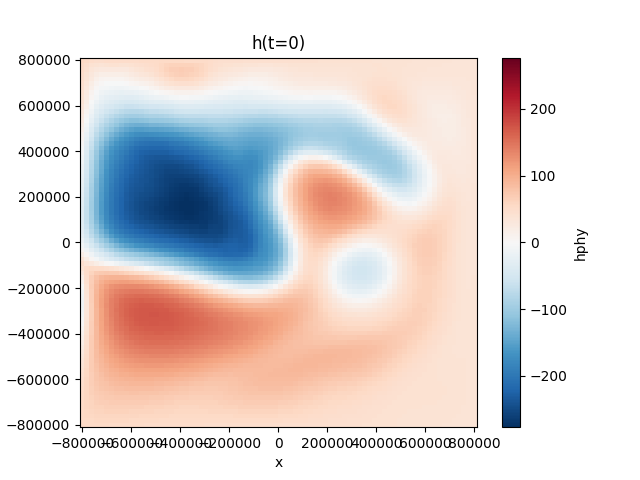
\includegraphics[width=\textwidth]{./fig/hinit.png}

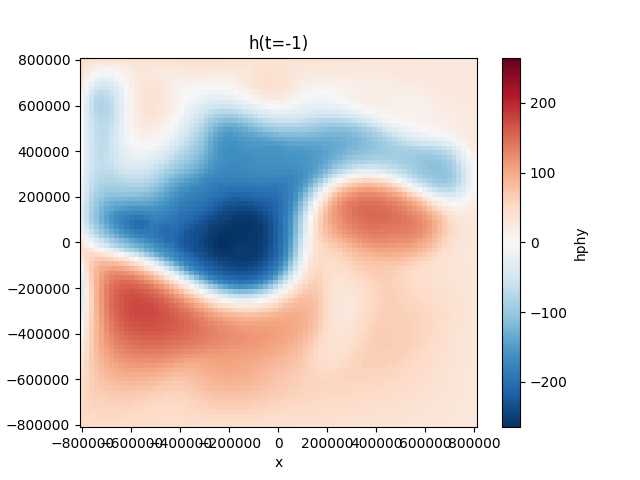
\includegraphics[width=\textwidth]{./fig/hfin.png}

\column{.3\textwidth}
\centering
u

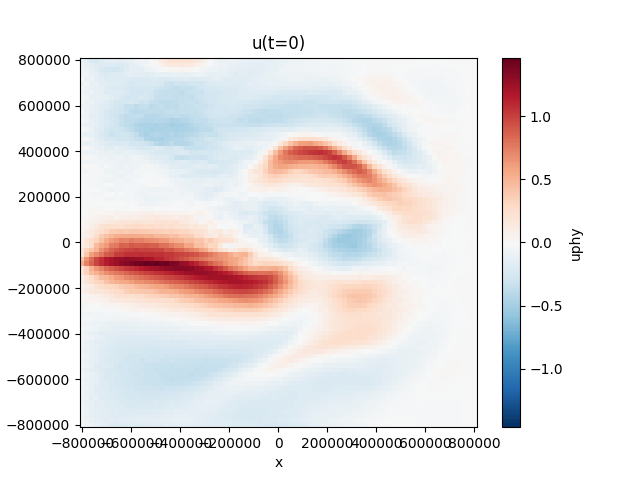
\includegraphics[width=\textwidth]{./fig/uinit.png}

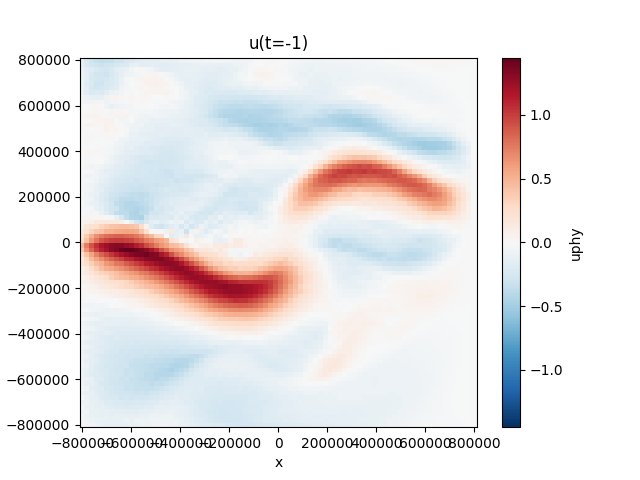
\includegraphics[width=\textwidth]{./fig/ufin.png}

\column{.3\textwidth}
\centering
v

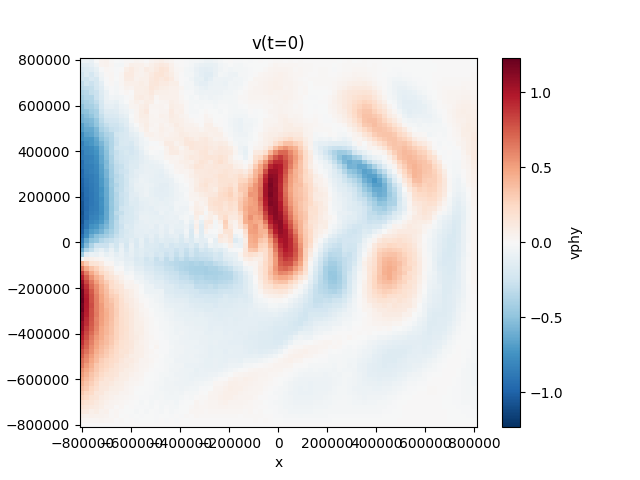
\includegraphics[width=\textwidth]{./fig/vinit.png}

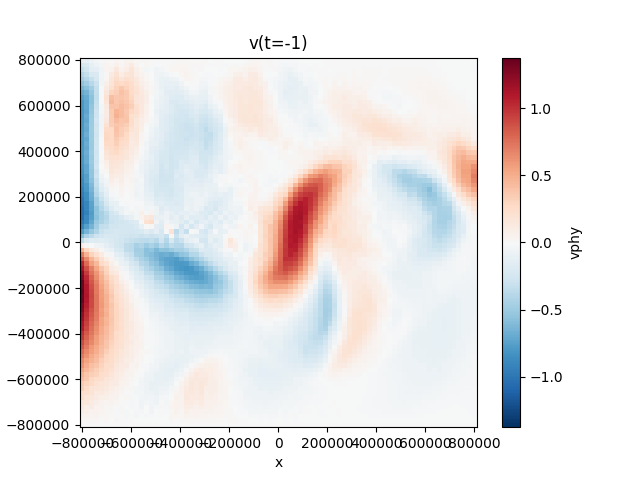
\includegraphics[width=\textwidth]{./fig/vfin.png}

\end{columns}
\end{frame}

%%%%%%%%%%%%%%%%%%%%
\begin{frame}
\frametitle{Some numerical artifacts ?}
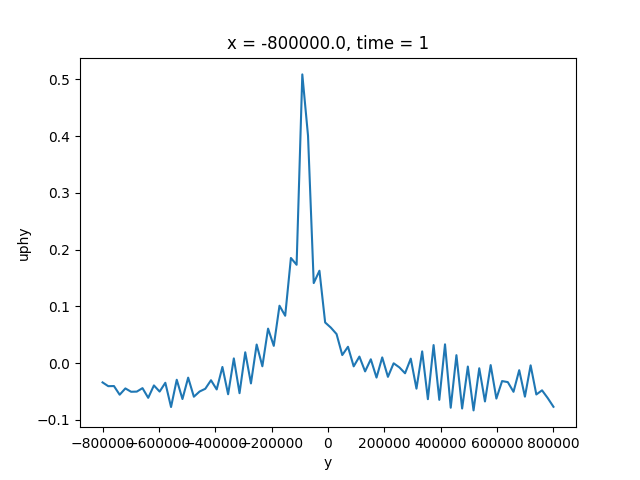
\includegraphics[height=.8\textheight]{./fig/transect_u_x0.png}
\end{frame}


%%%%%%%%%%%%%%%%%%%%
\begin{frame}
\frametitle{Principes of Neural Net aproach}
\tikzstyle{na} = [baseline=-.5ex]
\begin{eqnarray}
\partial_tu & = & 
\tikz[baseline]{\node[fill=blue!20,anchor=base] (udyn) {%
$+ (f + z ).v  - \partial_x (\frac{u^2+v^2}{2} + g^*.h) $} ;}
+
\tikz[baseline]{\node[fill=red!20,anchor=base] (upar) {%
$\frac{\tau_x}{\rho_0(H+h)} - \gamma . u + \nu\Delta u$} ;}\nonumber \\
\partial_tv & = & 
\tikz[baseline]{\node[fill=blue!20,anchor=base] (vdyn) {%
$- (f + z ).u  - \partial_y (\frac{u^2+v^2}{2} + g^*.h) $} ;}
+ 
\tikz[baseline]{\node[fill=red!20,anchor=base] (vpar) {%
$\frac{\tau_y}{\rho_0(H+h)} - \gamma . v + \nu\Delta v$} ;}\nonumber  \label{shal-nonlin-cs}\\
\partial_th & = & 
\tikz[baseline]{\node[fill=blue!20,anchor=base] (hdyn) {%
$- \partial_x(u(H+h)) - \partial_y(v(H+h))$};} \nonumber
\end{eqnarray}
\pause
New notation:
\begin{eqnarray}
\partial_tu & = & 
\tikz[baseline]{\node[fill=blue!20,anchor=base] (udyn) {%
udyn(u,v,h,f)} ;}
+
\tikz[baseline]{\node[fill=red!20,anchor=base] (upar) {%
upar(u,h,$\tau_x$,H)} ;}\nonumber \\
\partial_tv & = & 
\tikz[baseline]{\node[fill=blue!20,anchor=base] (vdyn) {%
vdyn(u,v,h,f)} ;}
+ 
\tikz[baseline]{\node[fill=red!20,anchor=base] (vpar) {%
vpar(v,h,$\tau_y$,H)} ;}\nonumber  \label{shal-nonlin-cs}\\
\partial_th & = & 
\tikz[baseline]{\node[fill=blue!20,anchor=base] (hdyn) {%
hdyn(u,v,h,H)};} \nonumber
\end{eqnarray}
\begin{block}{Idea}
substitute one of several process by a neural net
\end{block}
\end{frame}


%%%%%%%%%%%%%%%%%%%%
\begin{frame}
\frametitle{First attempt}
\begin{eqnarray}
\partial_tu & = & 
\tikz[baseline]{\node[fill=blue!20,anchor=base] (udyn) {%
udyn(u,v,h,f)} ;}
+
\tikz[baseline]{\node[fill=red!20,anchor=base] (upar) {%
upar$^{nn}$(u,h,$\tau_x$)} ;}\nonumber \\
\partial_tv & = & 
\tikz[baseline]{\node[fill=blue!20,anchor=base] (vdyn) {%
vdyn(u,v,h,f)} ;}
+ 
\tikz[baseline]{\node[fill=red!20,anchor=base] (vpar) {%
vpar$^{nn}$(v,h,$\tau_y$)} ;}\nonumber  \label{shal-nonlin-cs}\\
\partial_th & = & 
\tikz[baseline]{\node[fill=blue!20,anchor=base] (hdyn) {%
hdyn(u,v,h,H)};} \nonumber
\end{eqnarray}
H is considered constant

Neural nets are trained using a dataset of upar produced by a previous run of the complete numerical model.
\end{frame}


%%%%%%%%%%%%%%%%%%%%
\begin{frame}
\frametitle{Architecture of the neural net}
upar$^{nn}$ and vpar$^{nn}$ have the same architecture
\begin{enumerate}
\item Input : $u/v (3\times 3)$,$h (3\times 3)$,$\tau_{x/y} (3\times 3)$
\item CNN layer (relu) : 32 filters $(3\times 3) \rightarrow (1\times 1)$
\item "CNN" output layer (linear) : 1 filter $(1\times 1) \rightarrow (1\times 1)$

\end{enumerate}
\end{frame}


%%%%%%%%%%%%%%%%%%%%
\begin{frame}
\frametitle{Performance of the NN alone}
\begin{columns}
\column{.5\textwidth}
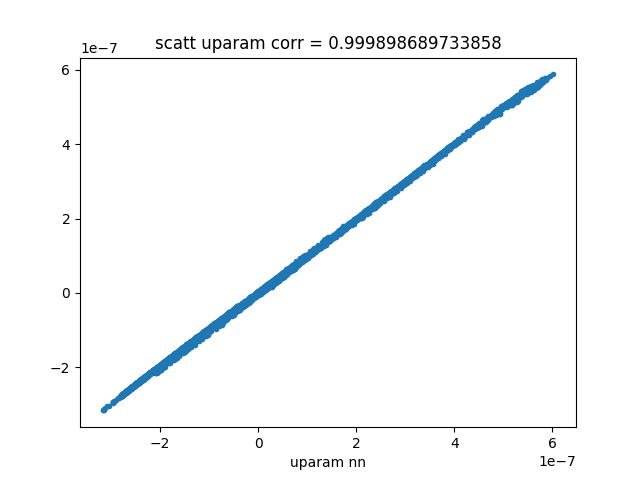
\includegraphics[width=\textwidth]{./fig/scat_upar.png}

\column{.5\textwidth}
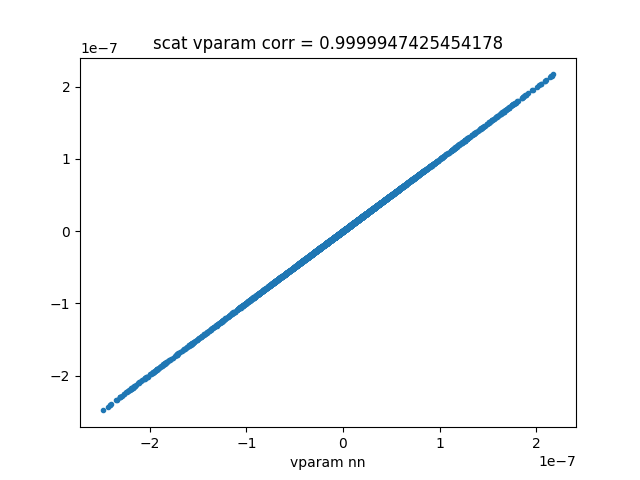
\includegraphics[width=\textwidth]{./fig/scat_vpar.png}

\end{columns}
\end{frame}


%%%%%%%%%%%%%%%%%%%%
\begin{frame}
\frametitle{Run of the NN model}
Make a one year run of the shallow-water model subsituting the nn model to the numerical model for
the upar, vpar calculation
\vspace{1em}

First difference : run time is much momre longer with the NN model (19 min Vs 7 sec)
\end{frame}

%%%%%%%%%%%%%%%%%%%%
\begin{frame}
\frametitle{Difference on fields}
\begin{columns}


\column{.32\textwidth}
\centering 
h

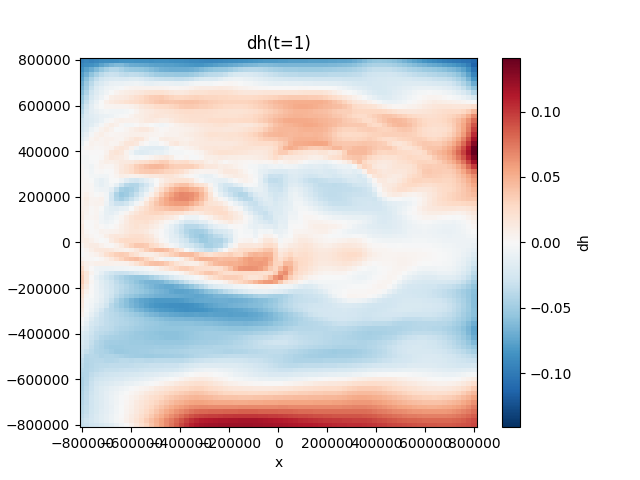
\includegraphics[width=\textwidth]{./fig/dhinit.png}

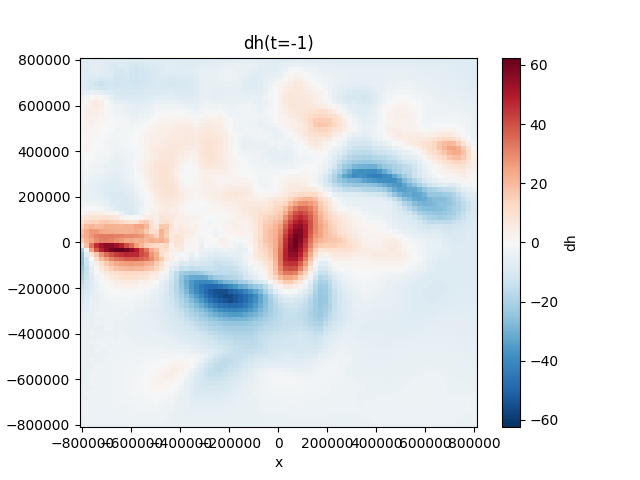
\includegraphics[width=\textwidth]{./fig/dhfin.png}
\column{.32\textwidth}
\centering 
u

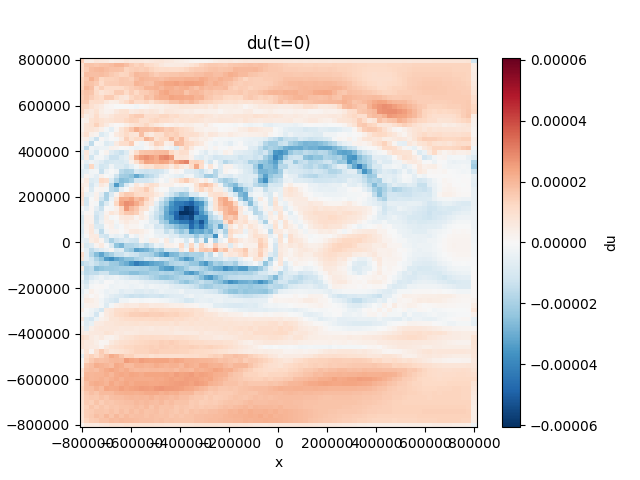
\includegraphics[width=\textwidth]{./fig/duinit.png}

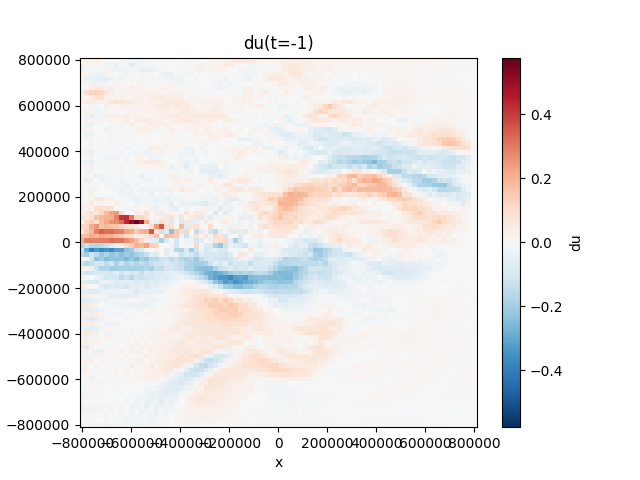
\includegraphics[width=\textwidth]{./fig/dufin.png}
\column{.32\textwidth}
\centering 
v

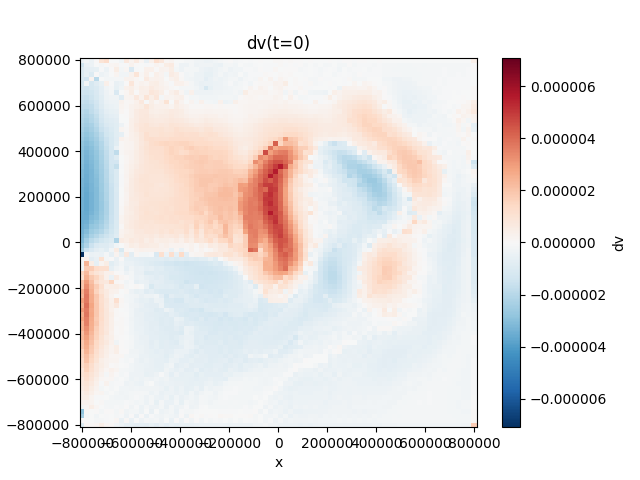
\includegraphics[width=\textwidth]{./fig/dvinit.png}

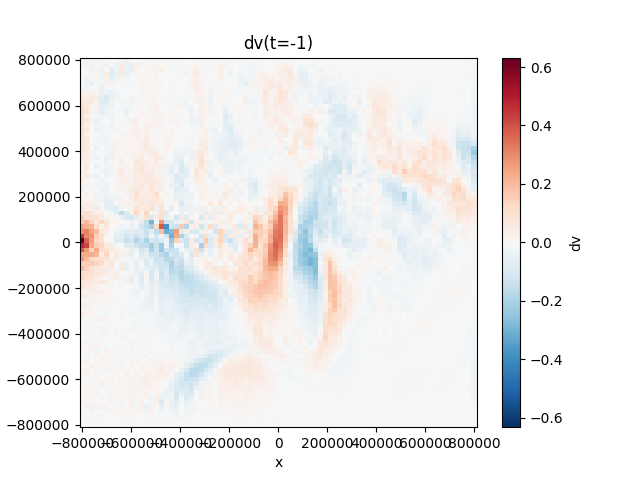
\includegraphics[width=\textwidth]{./fig/dvfin.png}
\end{columns}
\end{frame}
%%%%%%%%%%%%%%%%%%%%
\begin{frame}
\frametitle{Difference in time}
Evolution in time of point x = 10, y = 33
\begin{columns}

\column{.32\textwidth}
\centering 
h

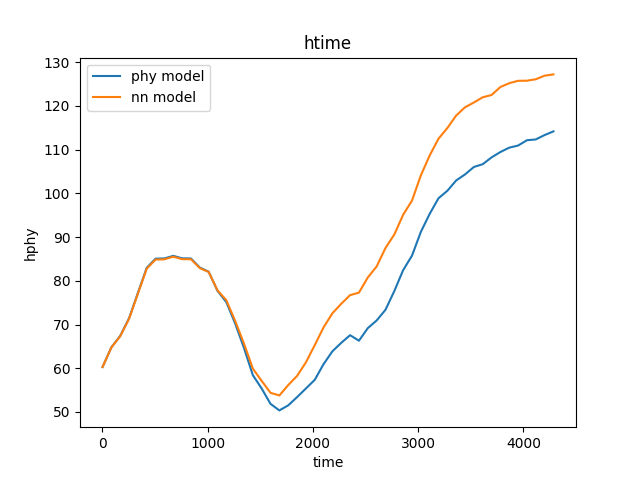
\includegraphics[width=\textwidth]{./fig/htime.png}

\column{.32\textwidth}
\centering 
u

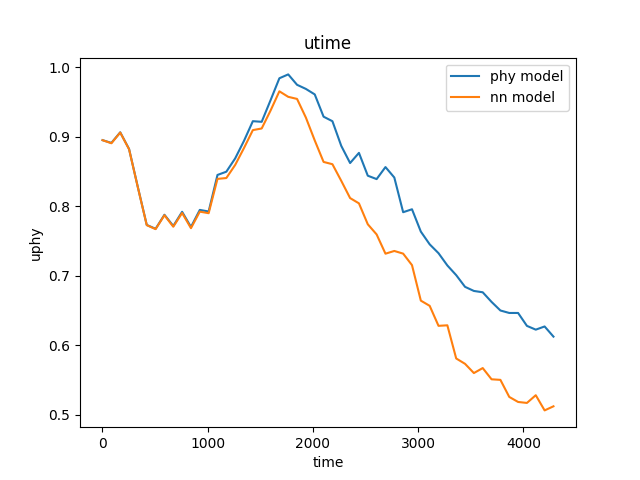
\includegraphics[width=\textwidth]{./fig/utime.png}

\column{.32\textwidth}
\centering 
v

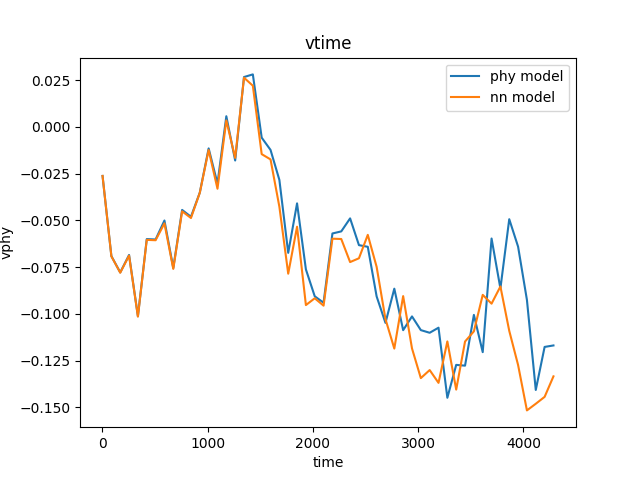
\includegraphics[width=\textwidth]{./fig/vtime.png}

\end{columns}

\end{frame}

%%%%%%%%%%%%%%%%%%%%
\begin{frame}
\frametitle{Difference in time}
Evolution in time of point x = 10, y = 33
\begin{columns}

\column{.5\textwidth}
\centering 
upar

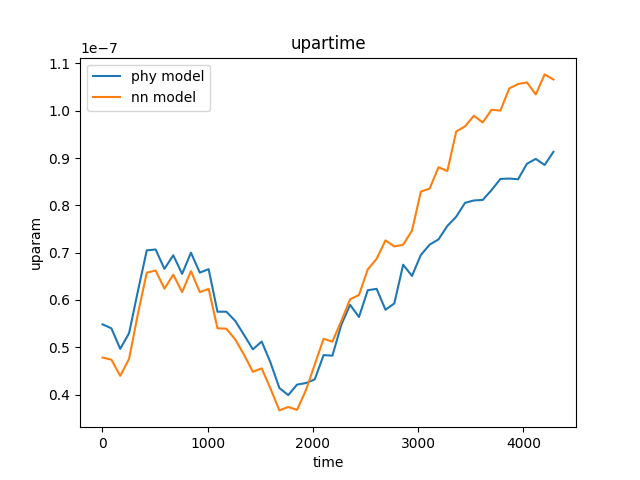
\includegraphics[width=\textwidth]{./fig/upartime.png}

\column{.5\textwidth}
\centering 
vpar

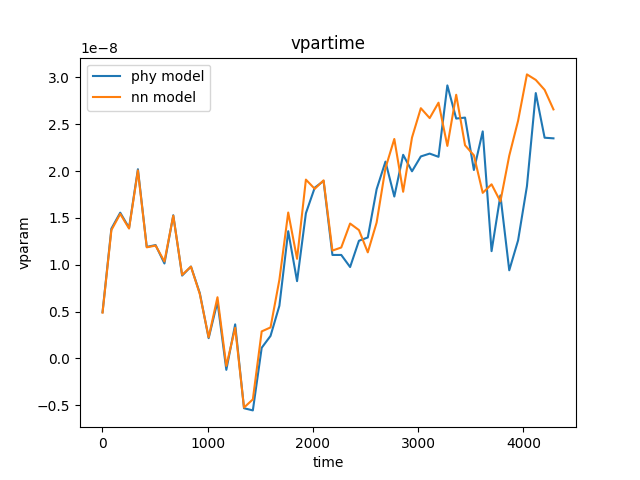
\includegraphics[width=\textwidth]{./fig/vpartime.png}


\end{columns}

\end{frame}
%%%%%%%%%%%%%%%%%%%%
\begin{frame}
\frametitle{Evolution of the RMS error}

\begin{columns}

\column{.32\textwidth}
\centering 
h

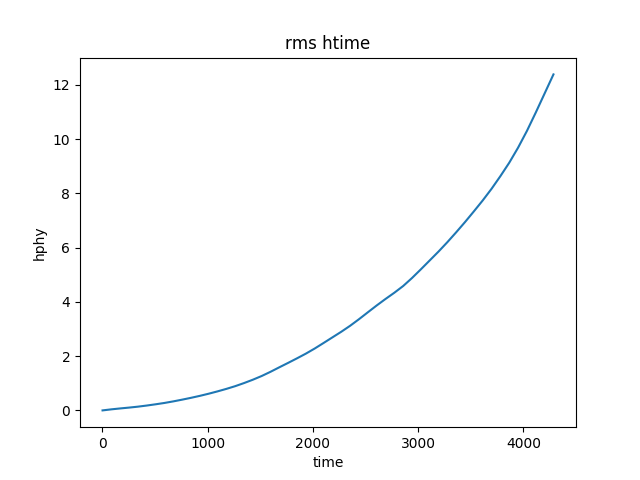
\includegraphics[width=\textwidth]{./fig/rms_htime.png}

\column{.32\textwidth}
\centering 
u

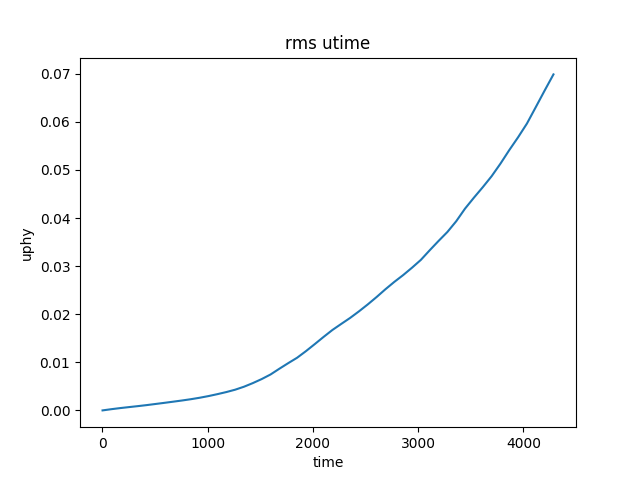
\includegraphics[width=\textwidth]{./fig/rms_utime.png}

\column{.32\textwidth}
\centering 
v

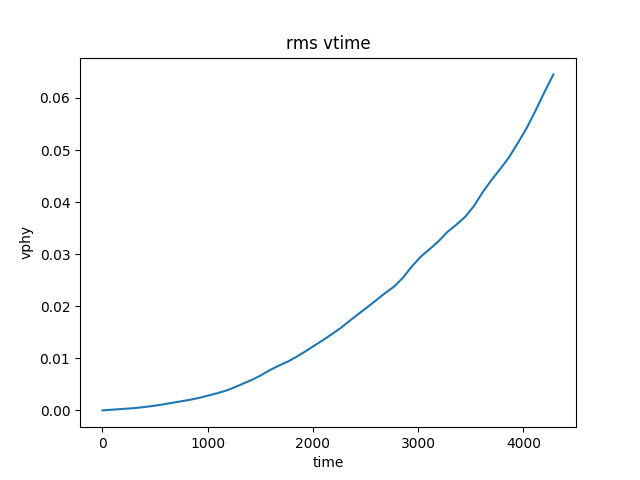
\includegraphics[width=\textwidth]{./fig/rms_vtime.png}

\end{columns}
\end{frame}
%%%%%%%%%%%%%%%%%%%%
\begin{frame}
\frametitle{RMS error on par}
Evolution in time of point x = 10, y = 33
\begin{columns}

\column{.5\textwidth}
\centering 
upar

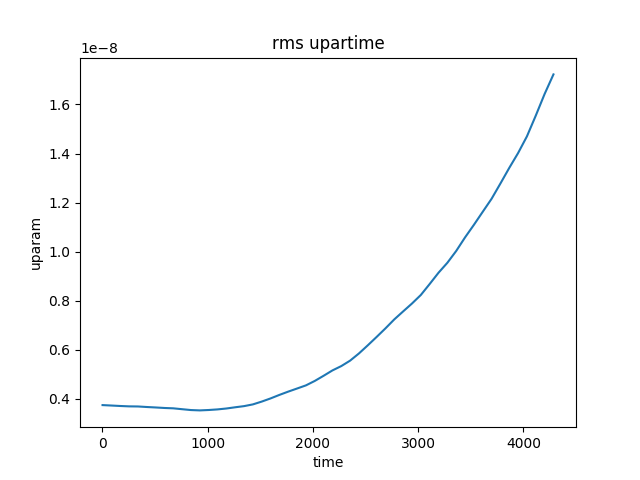
\includegraphics[width=\textwidth]{./fig/rms_upartime.png}

\column{.5\textwidth}
\centering 
vpar

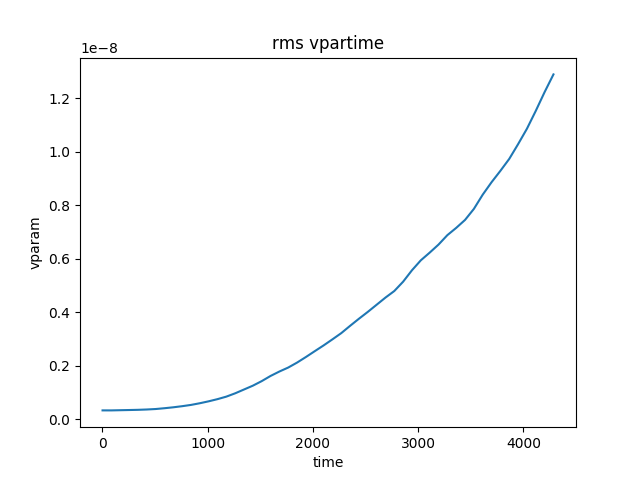
\includegraphics[width=\textwidth]{./fig/rms_vpartime.png}


\end{columns}

\end{frame}


%%%%%%%%%%%%%%%%%%%%
\begin{frame}
\frametitle{Next ?}
\begin{itemize}
\item Diags on the outputs ?
\item NN on the numerical core ?
\item Run on a high resolution model and learn on a coarser resolution ?
\end{itemize}
\end{frame}

\end{document}